\vspace{-0.5em}
\section{更引人入胜的观察} 
\label{sec:training_dynamics}
\vspace{-0.5em}

除了主要对比之外，我们还观察到一些有趣的现象，这些现象有助于更全面地了解半开放式路径检测（Semi-OPD）与开放式路径检测（OPD）之间的差异。更多有趣的观察结果见附录。

\noindent \textbf{同策略蒸馏（OPD）会收敛到由回放轨迹决定的平衡点，与初始化无关。}
一个自然的问题是：在半同策略蒸馏（Semi-OPD）之后，OPD 是否还能进一步提升性能？我们通过从 Semi-OPD 或教师回放蒸馏检查点进行初始化作为热启动来研究这一问题。如图~\ref{fig:handoff} 所示，在低重叠对中，无论初始值如何，所有实验最终均收敛至在相同回放上限下从初始学生模型初始化的 OPD 所达到的性能水平，而热启动仅影响收敛轨迹。  
相比之下，在高重叠对中，如图~\ref{fig:cache_switch_highoverlap} 所示，从 Semi-OPD 切换到 OPD 能够提升性能，并弥合了大部分与从零开始应用 OPD 的差距。  
这表明重复的同策略采样推动蒸馏趋向于由在线回放数据分布决定的平衡点，而非初始检查点。对该平衡点的刻画仍是未来工作的一个有趣方向。


\begin{figure}[h]
  \centering
  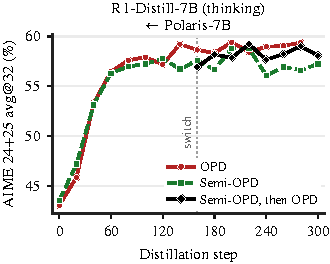
\includegraphics[width=0.8\linewidth]{figures/fig_cache_switch_polaris.pdf}
  \vspace{-0.5em}
  \caption{从半OPD切换到OPD，在重叠度较高的配对中，初始顶64重叠比为86.8\%时，可缩小与从头应用OPD的差距。}
  \label{fig:cache_switch_highoverlap}
\end{figure}


\noindent \textbf{收益会迁移到训练领域之外。}
如图~\ref{fig:code_transfer}所示，仅在数学密集型数据集~\citep{yu2025dapo}上蒸馏的模型在HumanEval和HumanEval+上也有所提升，且Semi-OPD仍然领先于OPD。
这表明这些收益并不局限于拟合数学训练分布，而是会迁移到更广泛的推理任务。


\begin{figure}[h]
  \centering
  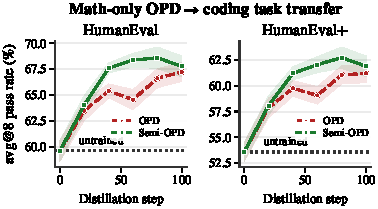
\includegraphics[width=\linewidth]{figures/fig_crossdomain.pdf}
  \vspace{-1.5em}
  \caption{\textbf{转换为代码。} 仅在数学上进行知识蒸馏的模型（Qwen3-1.7B $\leftarrow$  Qwen3-4B-Instruct-2507）的代码性能}
  \label{fig:code_transfer}
  \vspace{-1em}
\end{figure}

\begin{figure}[h]
  \centering
  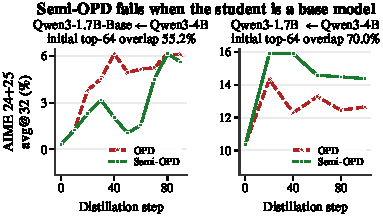
\includegraphics[width=\linewidth]{figures/fig_basestudent.pdf}
  \vspace{-1em}
   \caption{\textbf{初始学生能力。} 半OPD 与 OPD（相同教师），来自基础（左）和指令微调（右）的学生。}
    \label{fig:base_student}
    \vspace{-1em}
\end{figure}

\noindent \textbf{Semi-OPD 需要足够强的初始回溯轨迹。}  
由于 Semi-OPD 仅在来自 $\pi_0$ 的回溯轨迹上进行训练，因此初始回溯轨迹必须达到一定的质量阈值，才能实现有效的蒸馏。例如，如图~\ref{fig:base_student} 所示，使用基础学生模型时，初始回溯轨迹过于薄弱，导致 Semi-OPD 表现不如 OPD；而使用经过指令微调的学生模型时，Semi-OPD 重新展现出其优势。  
因此，当初始学生模型已能生成有意义的轨迹时，Semi-OPD 最为适用。